\section{Esercizio 7}

\textit{\textbf{Descrizione:} Calcolare la molteplicit\'a della radice nulla della funzione $f(x) = x^{2} \cdot sin(x^{2})$. Confrontare, quindi, i metodi di Newton, Newton modificato, e di Aitken, per approssimarla per gli stessi valori di tol del precedente esercizio (ed utilizzando il medesimo criterio di arresto), partendo da $x_{0}=1$. Tabulare e commentare i risultati ottenuti.}\\~\\
\emph{Soluzione:}\\~\\
La molteplicit\'a $m$ della radice nulla della funzione $f(x) = x^{2} \cdot sin(x^{2})$  \'e $m=4$
\\~\\

\textbf{il metodo di Newton modificato:}
\\~\\
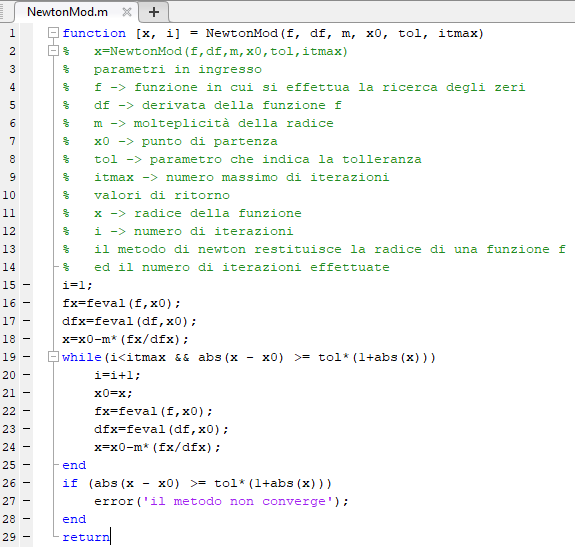
\includegraphics[width=1.3\linewidth]{img/NewtonMod}\newpage
\textbf{il metodo di aitken:}
\\~\\
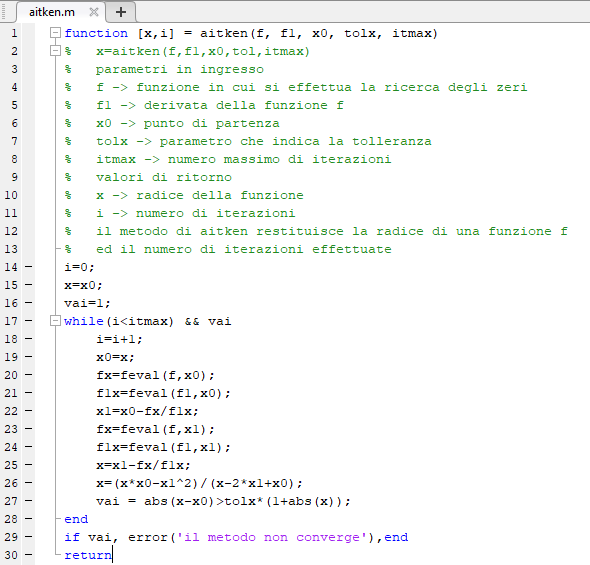
\includegraphics[width=1.3\linewidth]{img/aitken}\newpage
\makebox[\textwidth][c]{
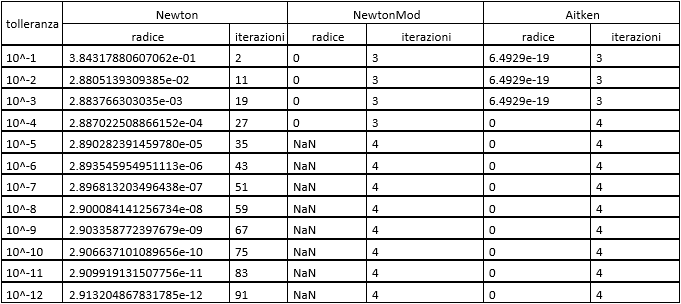
\includegraphics[width=1.3\textwidth]{img/tabella2}
}
